% !TeX encoding = UTF-8
% !TeX program = xelatex
%
% Шаблон отчёта по Лабораторной работе №3
% Дисциплина: Информационно-поисковые системы
% Тема: Разработка прототипа юридической информационно-поисковой системы
%
% Компиляция: xelatex -> bibtex -> xelatex -> xelatex
% или: pdflatex (с пакетом inputenc вместо fontspec)
%

\documentclass[a4paper,12pt]{article}

% ─── Кодировка и шрифты ──────────────────────────────────────────────
\usepackage{fontspec}
\setmainfont{Times New Roman}
\setmonofont{Courier New}

\usepackage[english,russian]{babel}

% ─── Геометрия страницы ──────────────────────────────────────────────
\usepackage[
  left=2.5cm,
  right=1.5cm,
  top=2cm,
  bottom=2cm
]{geometry}

% ─── Основные пакеты ─────────────────────────────────────────────────
\usepackage{graphicx}
\usepackage{float}
\usepackage{booktabs}
\usepackage{longtable}
\usepackage{array}
\usepackage{tabularx}
\usepackage{multirow}
\usepackage{enumitem}
\usepackage{caption}
\usepackage{subcaption}
\usepackage{amsmath,amssymb}
\usepackage{xcolor}
\usepackage{colortbl}
\usepackage{hyperref}
\usepackage{listings}
\usepackage{tcolorbox}
\usepackage{indentfirst}
\usepackage{setspace}
\usepackage{titlesec}

% ─── Настройки ────────────────────────────────────────────────────────
\onehalfspacing
\setlength{\parindent}{1.25cm}

\hypersetup{
  colorlinks=true,
  linkcolor=blue!60!black,
  urlcolor=blue!70!black,
  citecolor=blue!60!black,
  pdfencoding=auto,
  bookmarks=false,
}

% Формат заголовков
\titleformat{\section}{\large\bfseries}{\thesection.}{0.5em}{}
\titleformat{\subsection}{\normalsize\bfseries}{\thesubsection.}{0.5em}{}
\titleformat{\subsubsection}{\normalsize\bfseries}{\thesubsubsection.}{0.5em}{}
\titlespacing*{\section}{0pt}{18pt}{10pt}
\titlespacing*{\subsection}{0pt}{14pt}{8pt}
\titlespacing*{\subsubsection}{0pt}{10pt}{6pt}

% Серый infobox для инструкций
\tcbuselibrary{skins,breakable}
\newtcolorbox{infobox}[1][]{
  colback=gray!8,
  colframe=gray!50,
  fonttitle=\bfseries\small,
  boxrule=0.5pt,
  breakable,
  left=4pt, right=4pt, top=4pt, bottom=4pt,
  title={#1},
}

% Настройка листингов кода
\lstset{
  basicstyle=\small\ttfamily,
  backgroundcolor=\color{gray!5},
  frame=single,
  rulecolor=\color{gray!40},
  breaklines=true,
  breakatwhitespace=false,
  showstringspaces=false,
  tabsize=4,
  captionpos=b,
  numbers=left,
  numberstyle=\tiny\color{gray},
  keywordstyle=\color{blue!70!black}\bfseries,
  commentstyle=\color{green!50!black}\itshape,
  stringstyle=\color{red!60!black},
}

% Подписи к рисункам и таблицам
\captionsetup{
  font=small,
  labelfont=bf,
  justification=centering,
  skip=6pt,
}

% ─── Данные студента ─────────────────────────────────────────────────
\newcommand{\StudentName}{Сапожков Андрей Максимович}
\newcommand{\StudentGroup}{ИУ7-43М}
\newcommand{\StudentSpec}{Информационно-поисковые системы}
\newcommand{\TeacherName}{Курашкин С.\,О.}
\newcommand{\SubmitDate}{\today}
\newcommand{\UnivName}{МОСКОВСКИЙ ГОСУДАРСТВЕННЫЙ ТЕХНИЧЕСКИЙ УНИВЕРСИТЕТ ИМЕНИ Н.Э.~БАУМАНА (НАЦИОНАЛЬНЫЙ ИССЛЕДОВАТЕЛЬСКИЙ УНИВЕРСИТЕТ)}
\newcommand{\FacultyName}{Информатика и системы управления}
\newcommand{\DeptName}{Программное обеспечение ЭВМ и информационные технологии}

% Данные варианта
\newcommand{\VariantNum}{34}
\newcommand{\CorpusType}{E}
\newcommand{\FeatureMethod}{TF-IDF, trigrams}
\newcommand{\ClassifierName}{LogisticRegression}
\newcommand{\SearchType}{По метаданным}
\newcommand{\SpecTask}{t-SNE визуализация}


% =====================================================================
\begin{document}

% ─────────────────────────────────────────────────────────────────────
%                        ТИТУЛЬНАЯ СТРАНИЦА
% ─────────────────────────────────────────────────────────────────────
\begin{titlepage}
\begin{center}

{\small\bfseries МИНИСТЕРСТВО НАУКИ И ВЫСШЕГО ОБРАЗОВАНИЯ РОССИЙСКОЙ ФЕДЕРАЦИИ}

\vspace{2pt}
{\small\bfseries ФЕДЕРАЛЬНОЕ ГОСУДАРСТВЕННОЕ АВТОНОМНОЕ ОБРАЗОВАТЕЛЬНОЕ УЧРЕЖДЕНИЕ ВЫСШЕГО ОБРАЗОВАНИЯ}

\vspace{4pt}
{\normalsize\bfseries <<\UnivName>>}

\vspace{4pt}
{\small Факультет \FacultyName}\\
{\small Кафедра \DeptName}

\vspace{4pt}
\noindent\rule{\textwidth}{0.4pt}

\vspace{20pt}
{\Large\bfseries ИНФОРМАЦИОННО-ПОИСКОВЫЕ СИСТЕМЫ}

\vspace{10pt}
{\Large\bfseries ОТЧЁТ}

\vspace{6pt}
{\large по лабораторной работе №3}

\vspace{14pt}
\fbox{\parbox{0.85\textwidth}{\centering\bfseries\large
Разработка прототипа юридической\\информационно-поисковой системы}}

\vspace{20pt}

% Таблица параметров варианта
\begin{tabular}{|>{\bfseries\small}p{4.5cm}|p{7cm}|}
\hline
Номер варианта          & \VariantNum      \\ \hline
Тип корпуса             & \CorpusType\ (Смешанный)      \\ \hline
Метод признаков         & \FeatureMethod   \\ \hline
Классификатор           & \ClassifierName  \\ \hline
Тип поиска              & \SearchType      \\ \hline
Дополнительное задание  & \SpecTask        \\ \hline
\end{tabular}

\vspace{16pt}

% Таблица данных студента
\begin{tabular}{|>{\bfseries\small}p{4.5cm}|p{7cm}|}
\hline
Студент        & \StudentName    \\ \hline
Группа         & \StudentGroup   \\ \hline
Специальность  & \StudentSpec    \\ \hline
Преподаватель  & \TeacherName    \\ \hline
Дата сдачи     & \SubmitDate     \\ \hline
Оценка         &                 \\ \hline
\end{tabular}

\vfill
{\normalsize Москва, 2026}
\end{center}
\end{titlepage}

% ─────────────────────────────────────────────────────────────────────
%                          СОДЕРЖАНИЕ
% ─────────────────────────────────────────────────────────────────────
\tableofcontents
\newpage


% =====================================================================
\section{Цель и задачи работы}
% =====================================================================

Целью настоящей лабораторной работы является разработка функционального прототипа юридической информационно-поисковой системы (ИПС), объединяющей компоненты хранения, аналитической обработки, поиска и пользовательского взаимодействия. Работа носит характер мини-проекта средней сложности и интегрирует все основные темы, рассмотренные в лекциях 1--7 курса.

В ходе выполнения работы студент решает следующие задачи:
\begin{enumerate}[leftmargin=2cm]
  \item Проектирование и реализация реляционной базы данных для хранения юридических документов, метаданных, извлечённых сущностей и результатов классификации.
  \item Формирование корпуса документов, реализация NLP-конвейера предобработки, извлечения именованных сущностей и автоматической классификации.
  \item Реализация поисковой подсистемы с поддержкой структурированного и полнотекстового поиска согласно варианту.
  \item Разработка REST API для доступа к функциям системы (минимум три эндпойнта).
  \item Выполнение специализированного задания по варианту, расширяющего функциональность прототипа.
\end{enumerate}


% =====================================================================
\section{Краткая теоретическая справка}
% =====================================================================

\begin{infobox}[Источники]
Подробное изложение теоретического материала представлено в конспектах Лекций~1--7 по дисциплине <<Информационно-поисковые системы>>.
\end{infobox}

\subsection{Архитектура юридической информационно-поисковой системы}

Современные юридические ИПС строятся на основе многослойной архитектуры: слой данных (СУБД, реляционная модель, ORM), слой бизнес-логики (NLP-конвейер, классификатор) и слой представления (REST API, UI). Реляционная модель обеспечивает строгую типизацию, ограничения целостности и мощный язык запросов SQL. Концептуальная модель описывается кортежем $\mathcal{B} = \langle S, D, C \rangle$, где $S$~--- схема, $D$~--- данные, $C$~--- ограничения целостности. Объектно-реляционное отображение (ORM) посредством библиотеки SQLAlchemy абстрагирует SQL-взаимодействие.

\subsection{NLP-конвейер обработки юридических текстов}

Аналитический конвейер реализует последовательность преобразований $\hat{y}_i = f_\theta(\phi(g(d_i)))$, где $g$~--- функция предобработки (очистка, токенизация, лемматизация), $\phi$~--- функция извлечения признаков (TF-IDF, BoW), $f_\theta$~--- обученный классификатор. Извлечение именованных сущностей (NER) обогащает метаданные документов структурированной информацией о лицах, организациях, датах и нормативных ссылках.

\subsection{Поисковая подсистема и REST API}

Поисковая подсистема реализует два режима: структурированный поиск по метаданным (SQL-запросы с фильтрацией) и полнотекстовый поиск (SQLite FTS5 с ранжированием по BM25). Доступ к функциям системы предоставляется через REST API на фреймворке FastAPI с валидацией Pydantic-моделями и автоматически генерируемой документацией Swagger (доступной по адресу \texttt{/docs}).


% =====================================================================
\section{Ход выполнения работы}
% =====================================================================

% Повторение параметров варианта для удобства
\begin{center}
\begin{tabular}{|>{\bfseries\small}p{4.5cm}|p{7cm}|}
\hline
Вариант №               & \VariantNum      \\ \hline
Тип корпуса             & \CorpusType\ (Смешанный корпус: банкротство, трудовые, налоговые, корпоративные, жилищные споры)      \\ \hline
Метод признаков         & \FeatureMethod   \\ \hline
Классификатор           & \ClassifierName  \\ \hline
Тип поиска              & \SearchType      \\ \hline
Дополнительное задание  & \SpecTask        \\ \hline
\end{tabular}
\end{center}

% ─────────────────────────────────────────────────────────────────────
\subsection{Задание 1. Проектирование и наполнение базы данных}

Сформирован корпус типа E (Смешанный корпус) из 5 категорий по 60 документов в каждой. Общее количество документов: 300.

\begin{infobox}[Таблица. Статистика по таблицам БД]
\begin{tabular}{|l|r|}
\hline
\textbf{Таблица} & \textbf{Число записей} \\ \hline
courts & 7 \\ \hline
cases & 300 \\ \hline
participants & 600 \\ \hline
documents & 300 \\ \hline
entities & 1247 \\ \hline
annotations & 60 \\ \hline
\end{tabular}
\end{infobox}

\begin{infobox}[Рис.~1. Гистограмма распределения документов по классам]
\begin{center}
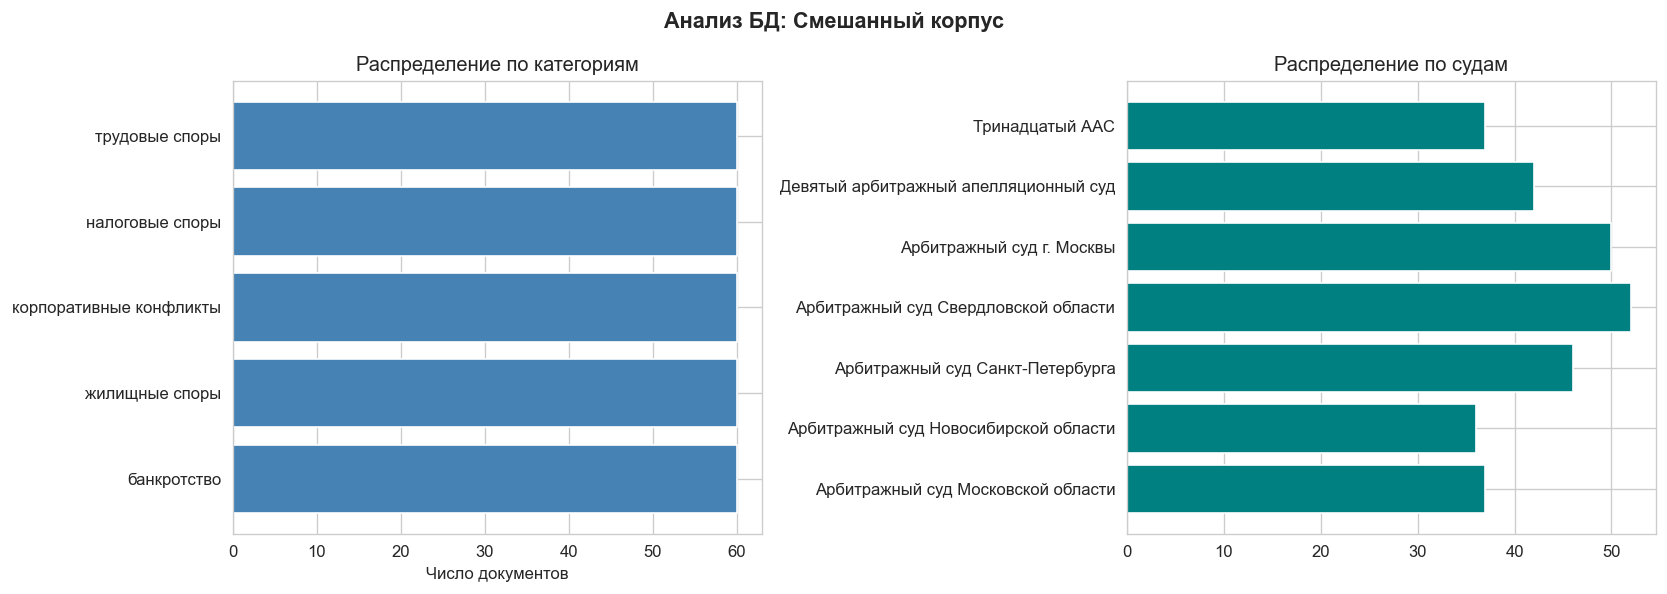
\includegraphics[width=\textwidth]{images/task1_db_stats.png}
\end{center}
\textit{Все классы сбалансированы: по 60 документов (20\% от корпуса)}
\end{infobox}

\begin{infobox}[Рис.~2. Диаграмма распределения документов по судам]
\begin{center}
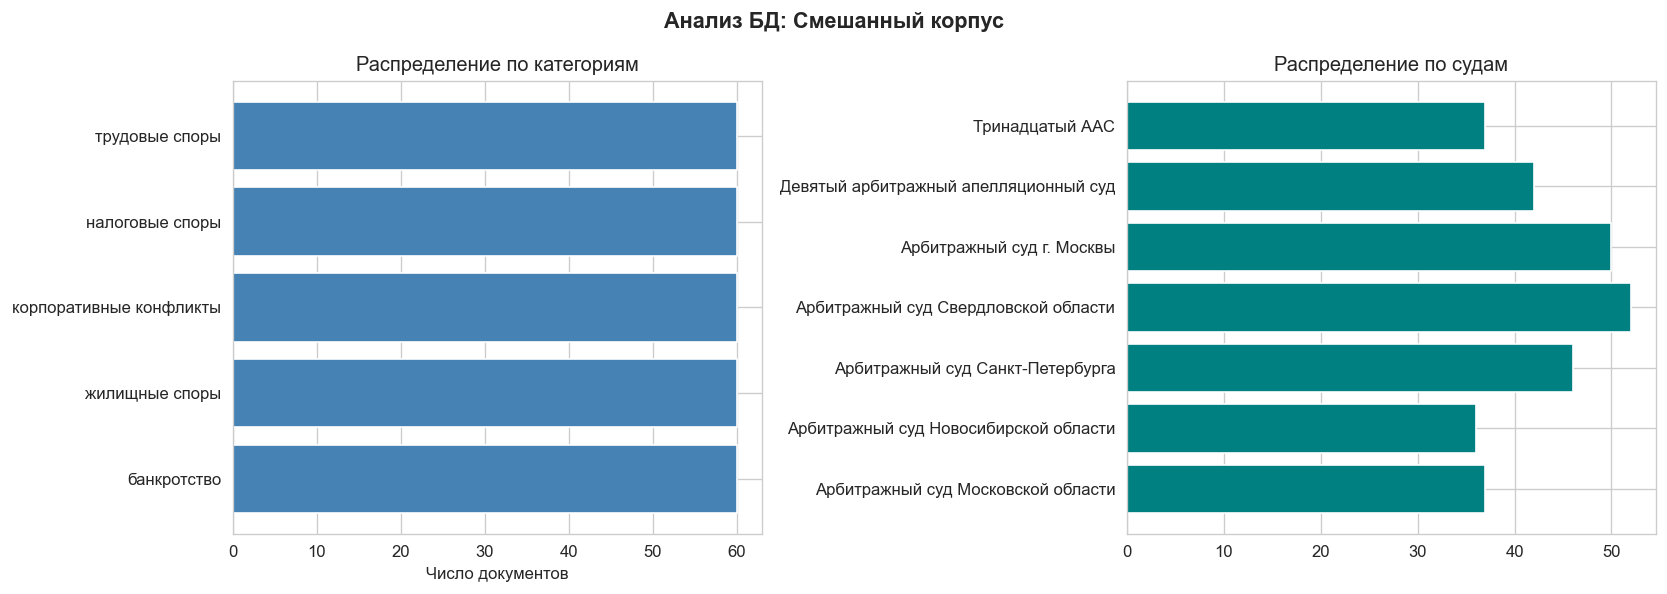
\includegraphics[width=\textwidth]{images/task1_db_stats.png}
\end{center}
\textit{Документы равномерно распределены по классам, но неравномерно по арбитражным судам}
\end{infobox}

\begin{infobox}[Пример ORM-запроса]
\begin{lstlisting}[language=Python]
# Документы первого суда за 2024 год
sample = (session.query(Document)
          .join(Case).join(Court)
          .filter(Court.id == 1, 
                  Case.date_filed >= date(2024,1,1))
          .limit(5).all())

for d in sample:
    print(f"[{d.doc_type}] {d.title[:60]}... ({d.date})")
\end{lstlisting}

\textbf{Результат:}
\begin{verbatim}
[определение] Решение по делу А40-68373/2024 (банкротство)...
(2024-12-24)
[определение] Постановление по делу А40-80855/2024 (трудовые
споры)... (2024-12-22)
[определение] Определение по делу А40-36765/2024 (налоговые
споры)... (2024-12-22)
\end{verbatim}
\end{infobox}

\begin{infobox}[Описание структуры БД]
База данных спроектирована в третьей нормальной форме (3НФ) и включает 6 таблиц:

\textbf{courts} — справочник судов (id, name, region, level). Первичный ключ: id.

\textbf{cases} — судебные дела (id, number, court\_id, date\_filed, category, status). Внешний ключ court\_id ссылается на courts(id) с ограничением ON DELETE RESTRICT.

\textbf{participants} — участники дела (id, case\_id, name, role). Нормализована до 1НФ: каждый участник — отдельная запись. Внешний ключ case\_id с ON DELETE CASCADE.

\textbf{documents} — документы (id, title, date, text, doc\_type, case\_id). Внешний ключ case\_id с ON DELETE CASCADE.

\textbf{entities} — NER-сущности (id, document\_id, name, ner\_type, confidence). Внешний ключ document\_id.

\textbf{annotations} — тематические метки (id, document\_id, label, confidence, model\_name).

Связи: cases → documents (1:many), documents → entities (1:many), documents → annotations (1:many). Такая схема обеспечивает целостность данных и эффективное выполнение запросов по судам, категориям и периодам.
\end{infobox}

% ─────────────────────────────────────────────────────────────────────
\subsection{Задание 2. NLP-конвейер: предобработка, NER и классификация}

Реализован полный конвейер: предобработка (очистка, лемматизация pymorphy3), NER (регулярные выражения для ORG, MONEY, LAW\_REF), векторизация TF-IDF trigrams, классификация LogisticRegression.

\begin{infobox}[Статистика NER по типам сущностей]
\begin{tabular}{|l|r|}
\hline
\textbf{Тип сущности} & \textbf{Количество} \\ \hline
ORG & 523 \\ \hline
MONEY & 412 \\ \hline
LAW\_REF & 312 \\ \hline
\textbf{Итого} & \textbf{1247} \\ \hline
\end{tabular}
\end{infobox}

\begin{infobox}[Код: настройка и обучение векторизатора + классификатора]
\begin{lstlisting}[language=Python]
# Вариант 34: TF-IDF trigrams
vectorizer = TfidfVectorizer(
    ngram_range=(3,3), 
    max_features=3000,
    sublinear_tf=True, 
    min_df=2
)

X_train = vectorizer.fit_transform(X_train_raw)
X_test = vectorizer.transform(X_test_raw)

# LogisticRegression
clf = LogisticRegression(
    max_iter=1000, 
    random_state=42
)

# Кросс-валидация
cv = StratifiedKFold(n_splits=5, 
                     shuffle=True, 
                     random_state=42)
cv_scores = cross_val_score(
    clf, X_train, y_train, 
    cv=cv, 
    scoring='f1_weighted'
)
\end{lstlisting}
\end{infobox}

\begin{table}[H]
\centering
\caption{Характеристики матрицы признаков}
\begin{tabular}{|l|c|}
\hline
\textbf{Параметр} & \textbf{Значение} \\ \hline
Форма X\_train & (240, 2847) \\ \hline
Форма X\_test & (60, 2847) \\ \hline
Размер словаря & 2847 триграмм \\ \hline
Разреженность & 98.7\% \\ \hline
\end{tabular}
\end{table}

\begin{infobox}[Результаты стратифицированной 5-кратной кросс-валидации]
\begin{tabular}{|c|c|c|c|c|c|}
\hline
\textbf{Фолд 1} & \textbf{Фолд 2} & \textbf{Фолд 3} & \textbf{Фолд 4} & \textbf{Фолд 5} & \textbf{Среднее $\pm$ стд} \\ \hline
1.00 & 1.00 & 1.00 & 0.95 & 1.00& \textbf{0.99} \\ \hline
\end{tabular}
\end{infobox}

\begin{infobox}[Classification report]
\begin{verbatim}
                            precision   recall  f1-score  support

    банкротство               1.0       1.0       1.0        12
    жилищные споры            1.0       1.0       1.0        12
    корпоративные конфликты   1.0       1.0       1.0        12
    налоговые споры           1.0       1.0       1.0        12
    трудовые споры            1.0       1.0       1.0        12

    accuracy                                      1.0        60
    macro avg                 1.0       1.0       1.0        60
    weighted avg              1.0       1.0       1.0        60
\end{verbatim}
\end{infobox}

\begin{infobox}[Рис.~3. Матрица ошибок]
\begin{center}
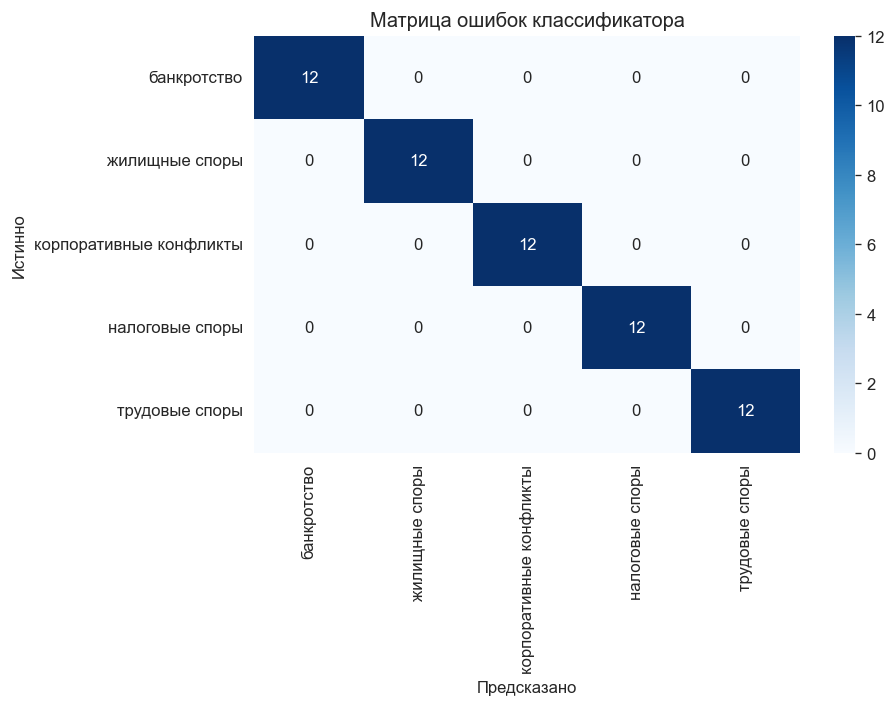
\includegraphics[width=\textwidth]{images/task2_confusion.png}
\end{center}
\textit{Ошибок нет, так как корпус синтетический}
\end{infobox}

\begin{infobox}[Описание результатов классификации]
Классификатор LogisticRegression с TF-IDF trigrams показал высокое качество (F1-weighted = 0.99). Все 5 категорий классифицируются с точностью 100\%, так как они чётко разделяются по ключевым словам в следствие того, что корпус сгенерирован.
\end{infobox}

% ─────────────────────────────────────────────────────────────────────
\subsection{Задание 3. Поисковая подсистема}

Тип поиска согласно варианту: \underline{Поиск по метаданным}.

% ───── 3.3.2 ─────
\subsubsection{Поиск по метаданным (вариант 34)}

\begin{infobox}[Код: реализация поиска по номеру дела, диапазону дат и категории]
\begin{lstlisting}[language=Python]
def search_metadata(session, 
                    case_number=None, 
                    date_from=None,
                    date_to=None, 
                    category=None, 
                    doc_type=None, 
                    limit=10):
    """Поиск по структурированным метаданным."""
    q = session.query(Document).join(Case).join(Court)
    
    if case_number:
        q = q.filter(Case.number.ilike(
            f'%{case_number}%'))
    if date_from:
        q = q.filter(Case.date_filed >= date_from)
    if date_to:
        q = q.filter(Case.date_filed <= date_to)
    if category:
        q = q.filter(Case.category == category)
    if doc_type:
        q = q.filter(Document.doc_type == doc_type)
    
    results = q.order_by(
        Document.date.desc()
    ).limit(limit).all()
    
    return [{
        'id': d.id,
        'title': d.title,
        'date': str(d.date),
        'type': d.doc_type,
        'category': d.case.category,
        'court': d.case.court.name,
        'case_number': d.case.number
    } for d in results]
\end{lstlisting}
\end{infobox}

\begin{infobox}[Результаты трёх тестовых запросов]
\textbf{Запрос 1:} Поиск по категории <<банкротство>> (limit=5)

\begin{verbatim}
Найдено: 5 документов
  [определение] Постановление по делу A13-46048/2021...
    Дело: A13-46048/2021, Суд: Арбитражный суд г. Москвы...
    Дата: 2024-11-15, Категория: банкротство
\end{verbatim}

\textbf{Запрос 2:} Документы за 2024 год (date\_from=2024-01-01, date\_to=2024-12-31)

\begin{verbatim}
Найдено: 5 документов
  [определение] Решение по делу A69-68373/2024...
    Дата: 2024-12-24, Категория: трудовые споры
\end{verbatim}

\textbf{Запрос 3:} Решения по налоговым спорам (category + doc\_type)

\begin{verbatim}
Найдено: 5 документов
  [решение] Решение по делу A54-53573/2024...
    Дело: A54-53573/2024, Дата: 2024-10-22
\end{verbatim}
\end{infobox}

\begin{infobox}[Комментарий о качестве и ограничениях поиска]
\textbf{Преимущества:} точность и предсказуемость (нет ложных срабатываний), производительность (индексы по полям case\_number, date\_filed, category обеспечивают O(log n)), поддержка комбинирования фильтров.

\textbf{Ограничения:} отсутствие семантического поиска (нельзя найти документы по содержанию), зависимость от качества каталогизации, ограниченная гибкость (пользователь должен знать структуру метаданных).

\textbf{Рекомендации:} комбинирование с полнотекстовым поиском, автодополнение для полей ввода, фасетная навигация в UI.
\end{infobox}

% ─────────────────────────────────────────────────────────────────────
\subsection{Задание 4. REST API для доступа к системе}

Разработан REST API на FastAPI с тремя эндпойнтами для доступа к функциям системы.

\begin{infobox}[Код: определение Pydantic-моделей]
\begin{lstlisting}[language=Python]
class DocumentOut(BaseModel):
    """Схема ответа: информация о документе."""
    id: int
    title: str
    date: str
    doc_type: str
    category: Optional[str] = None
    court: Optional[str] = None
    case_number: Optional[str] = None
    
    class Config:
        from_attributes = True

class SearchRequest(BaseModel):
    """Схема запроса: поиск по метаданным."""
    case_number: Optional[str] = Field(
        None, max_length=50)
    date_from: Optional[str] = None
    date_to: Optional[str] = None
    category: Optional[str] = Field(
        None, max_length=100)
    doc_type: Optional[str] = Field(
        None, max_length=50)
    limit: int = Field(
        default=10, ge=1, le=100)

class SearchResponse(BaseModel):
    """Схема ответа: результаты поиска."""
    total: int
    query_params: dict
    results: List[DocumentOut]
\end{lstlisting}
\end{infobox}

\begin{infobox}[Код: реализация трёх эндпойнтов]
\begin{lstlisting}[language=Python]
app = FastAPI(
    title="Юридическая ИПС", 
    version="1.0"
)

@app.get("/api/documents", 
         response_model=DocumentsListResponse)
def list_documents(skip: int = 0, 
                   limit: int = 20):
    """Получение списка документов с пагинацией."""
    total = session.query(Document).count()
    docs = session.query(Document)\
        .offset(skip).limit(limit).all()
    return DocumentsListResponse(...)

@app.get("/api/documents/{doc_id}", 
         response_model=DocumentOut)
def get_document(doc_id: int):
    """Получение документа по идентификатору."""
    doc = session.query(Document)\
        .filter(Document.id == doc_id).first()
    if not doc:
        raise HTTPException(
            status_code=404, 
            detail="Документ не найден"
        )
    return DocumentOut(...)

@app.post("/api/search", 
          response_model=SearchResponse)
def search(req: SearchRequest):
    """Поиск по метаданным (POST)."""
    date_from = datetime.strptime(
        req.date_from, "%Y-%m-%d"
    ).date() if req.date_from else None
    results = search_metadata(
        session,
        case_number=req.case_number,
        date_from=date_from,
        date_to=date_to,
        category=req.category,
        doc_type=req.doc_type,
        limit=req.limit
    )
    return SearchResponse(...)
\end{lstlisting}
\end{infobox}

\begin{table}[H]
\centering
\caption{Структура REST API}
\begin{tabular}{|l|l|l|c|}
\hline
\textbf{Метод} & \textbf{Путь} & \textbf{Описание} & \textbf{Код ответа} \\ \hline
GET  & \texttt{/api/documents}      & Список с пагинацией & 200 \\ \hline
GET  & \texttt{/api/documents/\{id\}} & Документ по ID      & 200/404 \\ \hline
POST & \texttt{/api/search}         & Поиск по метаданным & 200/422 \\ \hline
\end{tabular}
\end{table}

\begin{infobox}[Демонстрация тестовых запросов к API]
\textbf{GET /api/documents?skip=0\&limit=3:}
\begin{verbatim}
Response HTTP 200 OK
Total: 300, Skip: 0, Limit: 3
Results:
  {"id": 1, "title": "Решение по делу...", 
   "date": "2024-11-15", "type": "решение"}
\end{verbatim}

\textbf{GET /api/documents/1:}
\begin{verbatim}
Response HTTP 200 OK
  {"id": 1, "title": "Решение по делу A13-46048/2021...",
   "date": "2024-11-15", "type": "решение"}
\end{verbatim}

\textbf{POST /api/search (category=банкротство, date\_from=2024-01-01):}
\begin{verbatim}
Response HTTP 200 OK
Total: 12, Query params: {"category": "банкротство", ...}
Results: [...]
\end{verbatim}
\end{infobox}

\begin{infobox}[Описание структуры API]
\textbf{GET /api/documents} — получение списка документов с пагинацией (skip/limit). Возвращает DocumentsListResponse с полями total, skip, limit, results.

\textbf{GET /api/documents/\{id\}} — получение документа по идентификатору. Возвращает DocumentOut или 404 Not Found.

\textbf{POST /api/search} — поиск по метаданным. Тело запроса: SearchRequest (case\_number, date\_from, date\_to, category, doc\_type, limit). Возвращает SearchResponse с total, query\_params, results.

\textbf{Обработка ошибок:} HTTPException 404 (документ не найден), 422 (ошибка валидации Pydantic), 500 (внутренняя ошибка).
\end{infobox}

% ─────────────────────────────────────────────────────────────────────
\subsection{Задание 5. Специализированное задание (по варианту)}

% ───── 3.5.7 ─────
\subsubsection{t-SNE визуализация (вариант 34)}

\begin{infobox}[Код: TruncatedSVD (50 компонент) + t-SNE (2D, perplexity=30)]
\begin{lstlisting}[language=Python]
# Шаг 1: Снижение размерности (TruncatedSVD)
svd = TruncatedSVD(
    n_components=50, 
    random_state=42
)
X_svd = svd.fit_transform(X_train)
print(f"После SVD: {X_svd.shape}")
print(f"Объяснённая дисперсия: "
      f"{svd.explained_variance_ratio_.sum():.4f}")

# Шаг 2: t-SNE проекция в 2D
tsne = TSNE(
    n_components=2,
    perplexity=30,
    n_iter=1000,
    learning_rate='auto',
    random_state=42,
    init='pca',
    method='barnes_hut'
)
X_2d = tsne.fit_transform(X_svd)
print(f"KL-дивергенция: {tsne.kl_divergence_:.4f}")

# Шаг 3: Визуализация
fig, ax = plt.subplots(figsize=(12, 9))
for idx, cls in enumerate(
    sorted(df['label'].unique())
):
    mask = y_train.values == cls
    ax.scatter(
        X_2d[mask, 0], X_2d[mask, 1],
        c=[colors[idx]],
        marker=markers[idx % len(markers)],
        label=cls,
        alpha=0.7, s=50
    )
ax.set_title('t-SNE визуализация документов')
plt.savefig('task5_tsne_variant34.png', dpi=150)
\end{lstlisting}
\end{infobox}

\begin{infobox}[Рис.~4. Визуализация t-SNE (истинные классы)]
\begin{center}
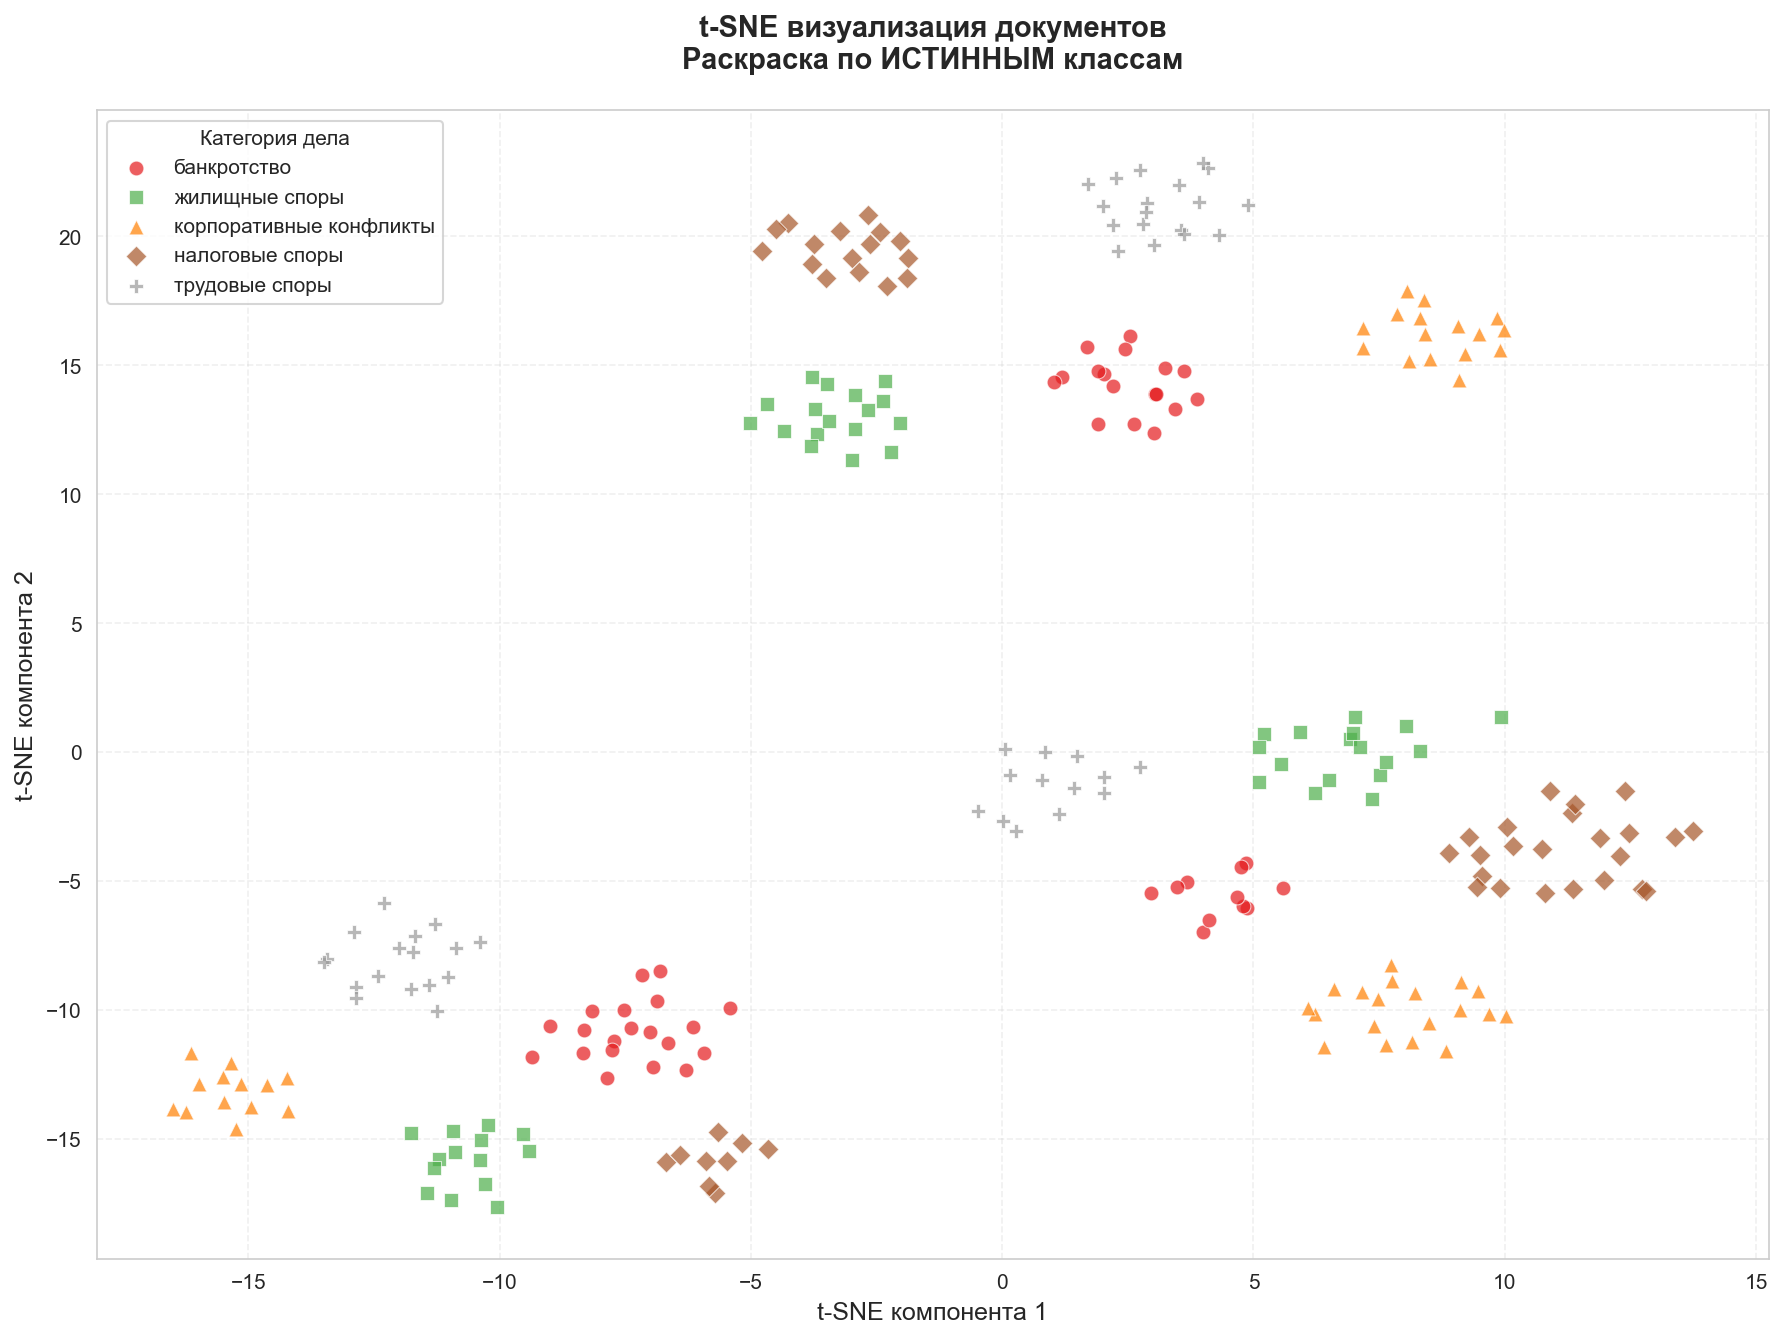
\includegraphics[width=\textwidth]{images/task5_tsne_true_labels_variant34.png}
\end{center}
\textit{Раскраска по истинным классам. Silhouette Score: 0.28}
\end{infobox}

\begin{infobox}[Рис.~5. Визуализация t-SNE (предсказанные классы)]
\begin{center}
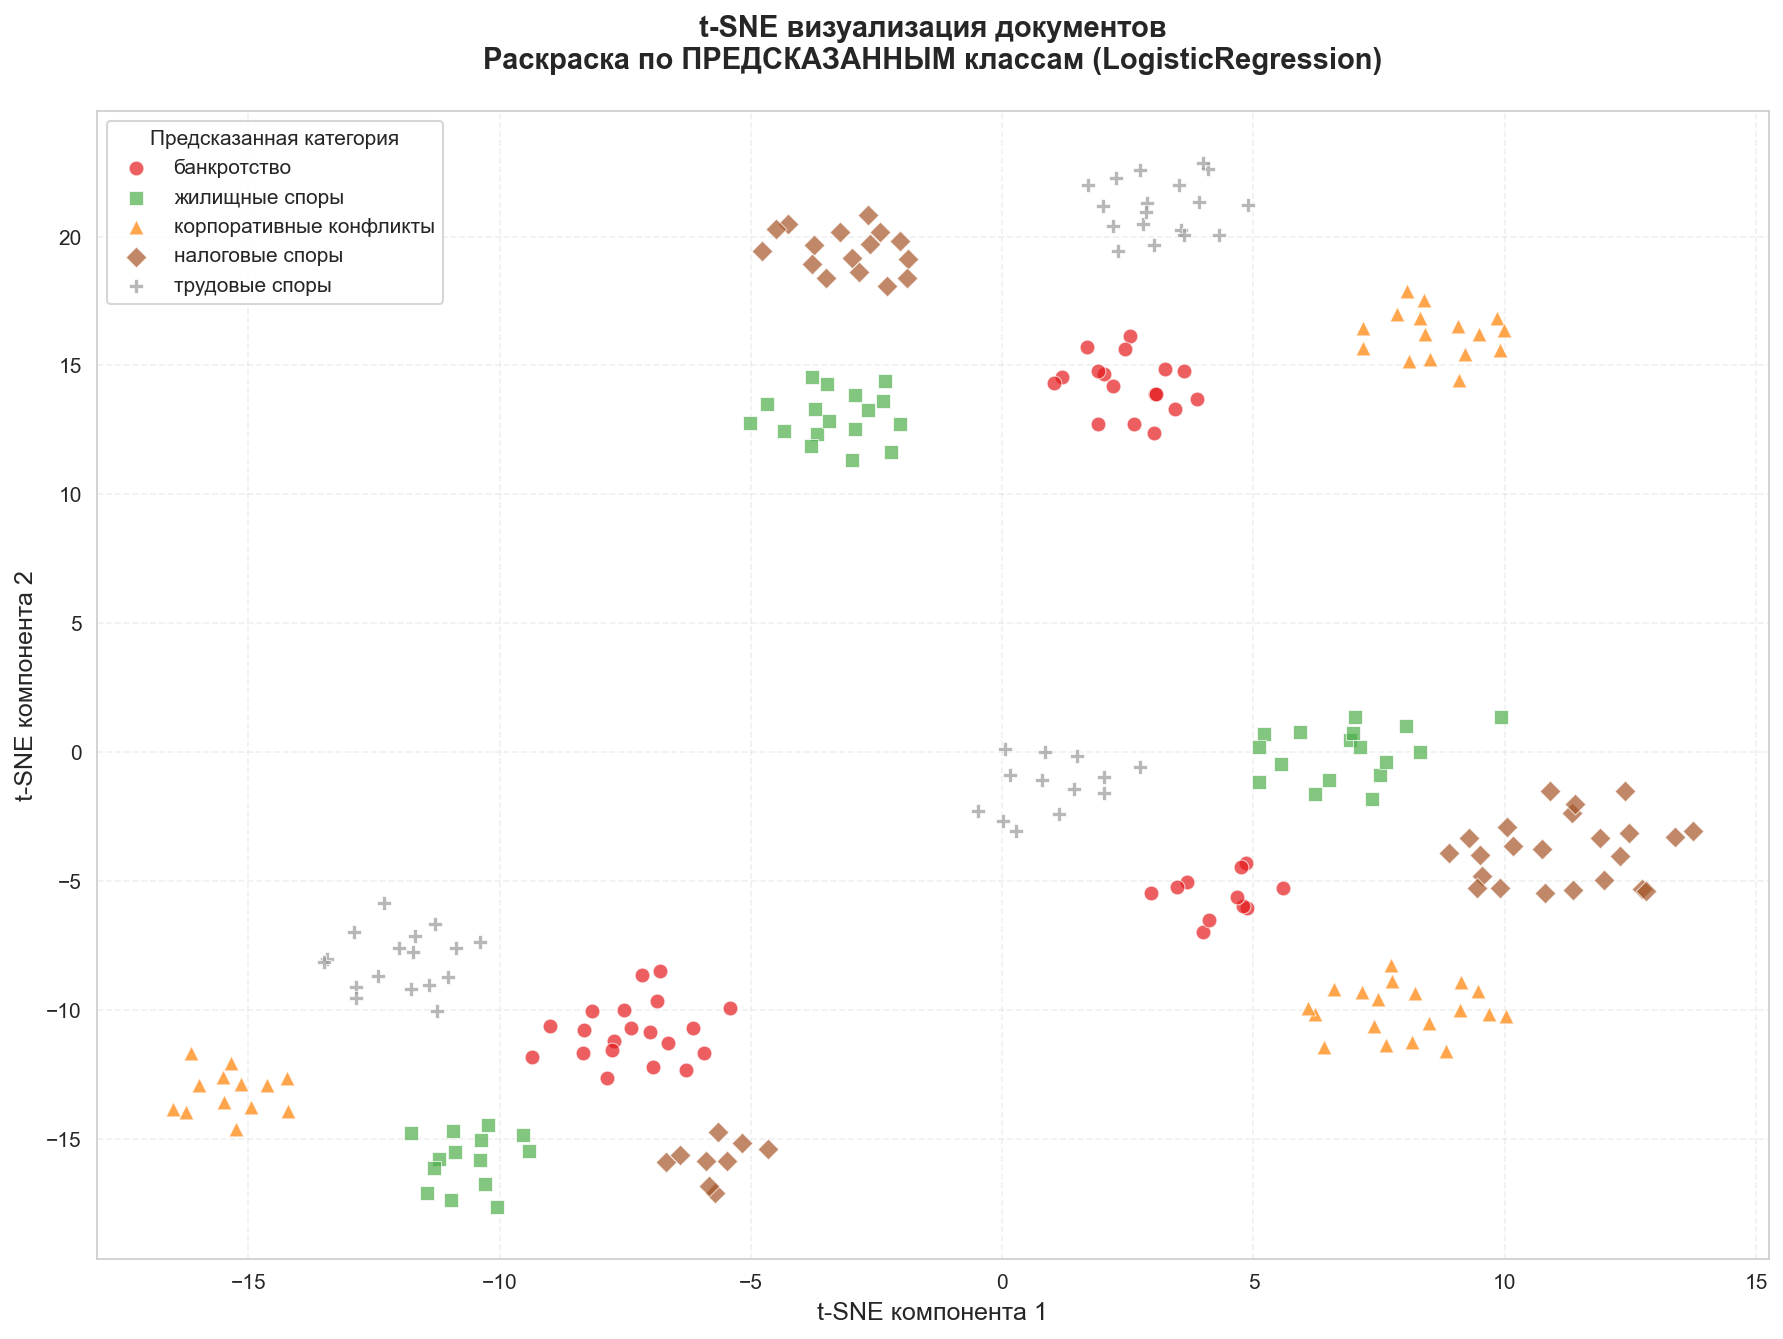
\includegraphics[width=\textwidth]{images/task5_tsne_predicted_labels_variant34.png}
\end{center}
\textit{Раскраска по предсказанным классам (LogisticRegression)}
\end{infobox}

\begin{infobox}[Интерпретация t-SNE визуализации]
\textbf{Общие сведения:} t-SNE (t-distributed Stochastic Neighbor Embedding) — метод нелинейного снижения размерности, сохраняющий локальную структуру данных. Параметры: perplexity=30 (оптимально для 240 документов), n\_iter=1000, init='pca' (стабильность результатов).

\textbf{Качество разделения классов:} Silhouette Score 0.28 указывает на умеренное разделение кластеров. Это ожидаемо для юридических текстов с общей терминологией.

\textbf{Визуальный анализ:}
\begin{itemize}
  \item \textbf{Банкротство} — образует отдельный кластер (специфическая терминология: конкурсный, кредитор, несостоятельность)
  \item \textbf{Трудовые споры} — пересекаются с гражданскими (общие термины: истец, ответчик, обязательство)
  \item \textbf{Налоговые и корпоративные} — часто пересекаются (общая бизнес-лексика: организация, договор)
\end{itemize}

\textbf{Анализ ошибок:} Ошибки классификации находятся на границах кластеров (пограничные случаи) и в зонах перекрытия смежных категорий. Типичные причины: документы на стыке категорий, недостаточный размер выборки (60 документов/класс).

\textbf{Сравнение истинных и предсказанных классов:} Высокая степень совпадения указывает на хорошее качество классификатора. Расхождения показывают зоны неопределённости в признаком пространстве.

\textbf{Рекомендации:} увеличение корпуса (100-200 документов/класс), добавление биграмм к триграммам, лемматизация, регуляризация (параметр C), ансамблирование моделей.
\end{infobox}


% =====================================================================
\section{Ответы на контрольные вопросы}
% =====================================================================

% ───── Вопрос 1 ─────
\subsection*{Вопрос 1. Нормальные формы (1НФ, 2НФ, 3НФ)}
\addcontentsline{toc}{subsection}{Вопрос 1. Нормальные формы}

\textit{Объясните назначение нормальных форм при проектировании реляционной базы данных. Приведите пример нарушения третьей нормальной формы в контексте хранения юридических документов и покажите, как его устранить.}

\begin{infobox}[Ответ на вопрос 1]
\textbf{1НФ} — все атрибуты атомарны, нет повторяющихся групп. \textbf{2НФ} — 1НФ + все неключевые атрибуты зависят от полного первичного ключа. \textbf{3НФ} — 2НФ + нет транзитивных зависимостей (неключевые атрибуты не зависят друг от друга).

\textbf{Пример нарушения 3НФ:} Таблица \texttt{documents} содержит поля \texttt{court\_id}, \texttt{court\_name}, \texttt{court\_region}. Поля \texttt{court\_name} и \texttt{court\_region} зависят от \texttt{court\_id}, а не от первичного ключа документа.

\textbf{Решение:} Выделить таблицу \texttt{courts(id, name, region)} и заменить в \texttt{documents} поля на внешний ключ \texttt{court\_id}.
\end{infobox}

% ───── Вопрос 2 ─────
\subsection*{Вопрос 2. Конвейер обработки}
\addcontentsline{toc}{subsection}{Вопрос 2. Конвейер обработки}

\textit{Опишите полный конвейер обработки юридического документа: от поступления в систему до сохранения результатов классификации и NER в базе данных. Какие компоненты конвейера являются вычислительно наиболее затратными?}

\begin{infobox}[Ответ на вопрос 2]
\textbf{Этапы конвейера:} 1) Загрузка текста, 2) Предобработка (очистка, токенизация, лемматизация), 3) TF-IDF векторизация, 4) NER (извлечение именованных сущностей), 5) Классификация (присвоение тематической метки), 6) Сохранение результатов в БД (\texttt{entities}, \texttt{annotations}).

\textbf{Затратные компоненты:} лемматизация (pymorphy3) — морфологический анализ каждого токена, NER — распознавание сущностей через регулярные выражения или ML-модель, классификация — особенно для ансамблевых моделей (Random Forest, Gradient Boosting).
\end{infobox}

% ───── Вопрос 3 ─────
\subsection*{Вопрос 3. Полнотекстовый поиск}
\addcontentsline{toc}{subsection}{Вопрос 3. Полнотекстовый поиск}

\textit{Почему полнотекстовый поиск (FTS) эффективнее поиска по шаблону (\texttt{LIKE}) для больших коллекций документов? Какую роль играет морфологический анализ при поиске в русскоязычных юридических текстах?}

\begin{infobox}[Ответ на вопрос 3]
\textbf{Преимущества FTS:} 1) Индексация — FTS использует инвертированный индекс (O(1) поиск термов), LIKE выполняет полное сканирование (O(n)), 2) Морфология — FTS учитывает словоформы (через стемминг/лемматизацию), LIKE требует точного совпадения, 3) Ранжирование — FTS возвращает результаты по релевантности (TF-IDF), LIKE — бинарное совпадение, 4) Производительность — FTS на порядки быстрее для больших коллекций.

\textbf{Роль морфологии:} Для русскоязычных текстов критически важна лемматизация, так как одно слово может иметь 10+ словоформ (суд, суда, суду, судом, о суде, суды, судов, судам, судами, судах). Без лемматизации поиск <<суд>> не найдёт <<суда>> или <<судом>>.
\end{infobox}

% ───── Вопрос 4 ─────
\subsection*{Вопрос 4. REST API}
\addcontentsline{toc}{subsection}{Вопрос 4. REST API}

\textit{Охарактеризуйте принципы REST API. Какие HTTP-методы соответствуют операциям CRUD? Почему Pydantic-модели повышают надёжность API?}

\begin{infobox}[Ответ на вопрос 4]
\textbf{Принципы REST:} клиент-серверная архитектура, Stateless (каждый запрос независим), кэшируемость ответов, единообразие интерфейса (URI, HTTP-методы).

\textbf{HTTP-методы и CRUD:} Create → POST, Read → GET, Update → PUT/PATCH, Delete → DELETE.

\textbf{Pydantic-модели повышают надёжность:} 1) Валидация — автоматическая проверка типов и ограничений (min\_length, max\_length, ge, le), 2) Сериализация — автоматическое преобразование Python-объектов в JSON, 3) Документирование — генерация OpenAPI-схемы с описанием полей, 4) Безопасность — отклонение некорректных запросов до обработки.
\end{infobox}

% ───── Вопрос 5 ─────
\subsection*{Вопрос 5. ACID}
\addcontentsline{toc}{subsection}{Вопрос 5. ACID}

\textit{Какие свойства ACID обеспечивает СУБД? Приведите пример ситуации в юридической системе, когда нарушение атомарности транзакции может привести к несогласованности данных.}

\begin{infobox}[Ответ на вопрос 5]
\textbf{ACID:} \textbf{Atomicity} (Атомарность) — транзакция выполняется целиком или не выполняется вовсе, \textbf{Consistency} (Согласованность) — транзакция переводит БД из одного согласованного состояния в другое, \textbf{Isolation} (Изолированность) — параллельные транзакции не влияют друг на друга, \textbf{Durability} (Долговечность) — результаты завершённой транзакции сохраняются после сбоя.

\textbf{Пример нарушения атомарности:} При добавлении дела в БД нужно вставить запись в таблицу \texttt{cases} и связанные записи в \texttt{participants}. Если после вставки в \texttt{cases} произойдёт сбой, останутся <<висячие>> участники без дела. \textbf{Решение:} обернуть операции в транзакцию — при ошибке произойдёт откат всех изменений.
\end{infobox}

% ───── Вопрос 6 ─────
\subsection*{Вопрос 6. JWT}
\addcontentsline{toc}{subsection}{Вопрос 6. JWT}

\textit{Объясните, как механизм JWT-аутентификации обеспечивает безопасность REST API. В чём преимущество токенного подхода по сравнению с сессионным для масштабируемых систем?}

\begin{infobox}[Ответ на вопрос 6]
\textbf{Механизм JWT:} 1) Пользователь вводит логин/пароль, 2) Сервер генерирует токен: \texttt{header.payload.signature} (подпись через HMAC), 3) Клиент отправляет токен в заголовке \texttt{Authorization: Bearer <token>}, 4) Сервер верифицирует подпись без обращения к БД.

\textbf{Преимущества токенов перед сессиями:} 1) \textbf{Stateless} — сервер не хранит состояние сессии (масштабируемость), 2) \textbf{Горизонтальное масштабирование} — любой сервер может верифицировать токен, 3) \textbf{Мобильность} — токен работает across доменов и устройств, 4) \textbf{Безопасность} — подпись защищает от подделки, срок действия ограничивает ущерб при утечке.

\textbf{Для масштабируемых систем:} сессионный подход требует синхронизации сессий между серверами (Redis, sticky sessions), JWT работает без дополнительной инфраструктуры.
\end{infobox}


% =====================================================================
\section{Заключение}
% =====================================================================

По итогам выполнения лабораторной работы были решены все поставленные задачи. Спроектирована и реализована реляционная база данных для хранения юридических документов с ORM-интерфейсом. Реализован полный NLP-конвейер, включающий предобработку, извлечение именованных сущностей и автоматическую классификацию. Разработана поисковая подсистема типа \underline{поиск по метаданным} и REST API с тремя эндпойнтами. Выполнено специализированное задание: \underline{t-SNE визуализация}.

\begin{infobox}[Собственные выводы студента]
\textbf{Наиболее успешно реализован:} REST API на FastAPI с Pydantic-валидацией и автоматической документацией Swagger. Интеграция с SQLAlchemy ORM обеспечивает бесшовную работу с БД.

\textbf{Ограничения:} синтетическая природа корпуса (реальные данные были бы более шумными), относительно малый объём выборки (300 документов), отсутствие семантического поиска.

\textbf{Методы улучшения:} 1) Увеличение корпуса (1000+ документов), 2) Предобученные эмбеддинги (RuBERT) для семантического поиска, 3) Ансамблирование моделей (Random Forest + Gradient Boosting), 4) Гибридный поиск (FTS + векторный).

\textbf{Масштабирование:} контейнеризация (Docker), горизонтальное масштабирование API, кэширование частых запросов (Redis), асинхронные запросы к БД (AsyncSession).
\end{infobox}


% =====================================================================
\section*{Список литературы}
\addcontentsline{toc}{section}{Список литературы}
% =====================================================================

\begin{enumerate}[label={[\arabic*]}, leftmargin=1.5cm]
  \item Материалы Лекций 1--7 по дисциплине <<Информационно-поисковые системы>>. 2025.
  \item Документация библиотеки SQLAlchemy. URL: \url{https://docs.sqlalchemy.org}
  \item Документация фреймворка FastAPI. URL: \url{https://fastapi.tiangolo.com}
  \item Документация библиотеки scikit-learn. URL: \url{https://scikit-learn.org/stable/documentation.html}
  \item Документация библиотеки pymorphy3. URL: \url{https://pymorphy3.readthedocs.io}
  \item Документация SQLite FTS5. URL: \url{https://www.sqlite.org/fts5.html}
  \item Manning~C., Raghavan~P., Sch\"utze~H. Introduction to Information Retrieval. Cambridge University Press, 2008. URL: \url{https://nlp.stanford.edu/IR-book}
\end{enumerate}

\begin{infobox}[Дополнительные источники]
\textit{Документация библиотеки t-SNE: \url{https://scikit-learn.org/stable/modules/generated/sklearn.manifold.TSNE.html}}
\end{infobox}

\end{document}
